\cleardoublepage
\chapter{Video Compression Systems}\label{chap:av1}

%%%%%%%%%%%%%%%%%%%%%%%%%%%%%%%%%%%%%%%%%%%%%%%%%%%%%%%%%%%%%%%%%%%%%%%%%%%%%%
\section{Basic Principles}

\emph{Video Compression Systems} have been in development for approximately forty years, with the first video codec, \emph{H.120}, being released in 1984. It was composed of basic operations, which didn't correlate to good compression performances. This has lead to a quick downfall of its usage, being aggravated by the release of the \emph{H.261} standard by 1984.

However, the building blocks on which later standards were based are the same as in the first generations, i.e., the strategies implemented on newer standards exploit the same \emph{redundancies} as previous, less efficient, codecs.

By redundancies, it is meant disposable information to the playback of an image sequence. This concept is the key of video compression. Throughout the years, the enhancement of video codecs was based on the improving the algorithms which can reliably represent a video, while maintaining the least of the original information. In other words, the video sequence is analyzed for predictable/identifiable characteristics, e.g. the movement of a subject or the edge of an object, calculates strategies of predicting nearby pixel values through that information and disposes the unused information. This process is mentioned as \emph{redundancy removal}.

This way, to have a better understanding of the functioning behind video codecs, the mentioned redundancies, and respective origins, are presented. Most of such have origin on the way humans perceive vision, being this the first topic of this chapter.

%%%%%%%%%%%%%%%%%%%%%%%%%%%%%%%%%%%%%%%
\subsection{Human Visual System} \label{ssec:hvs}

%\todo[inline,color=green!40]{*Essency of video compression relies on making changes the image without serious perception by the user}
%\todo[inline,color=green!40]{*Eye Functioning}
%\todo[inline,color=red!40]{*"Known Issues" (lower perception to chroma, high frequencies, etc)}
%\todo[inline,color=red!40]{*Opportunity to explore various types of redundancies to the image}

\nocite{gonzalezDigitalImageProcessing2018}

Most of the compressed/decompressed video nowadays is directed to content visualization by consumers, with the exception of some network-driven image processing applications, such as automatic video surveillance. Therefore, the compression of video sequences has the intent of making changes to the original data, without serious impact to the users' perception. This process is mentioned as the removal of the \emph{Psychovisual redundancy} \cite{shiImageVideoCompression2008}. Therefore, a basic understanding of the visual system can clarify many of the design choices made in video compression applications, and why their use doesn't present much impact on the quality of the image, while greatly reducing its size.

The image perception starts in the human eye, represented in figure \ref{fig:eye}. Its different constituents accomplish different tasks, from focusing, to aperture control. Although their importance to the overall functioning of the eye, the part that matters most to the focus of this work is the innermost membrane, the retina.

\begin{figure}[h]
    \centering
    \includegraphics[width=\figwidth]{Sections/2AV1/Diagrams/eyediagram.png}
    \caption[Representation of an human eye]{Representation of an human eye \cite{AnatomyEyeHuman}}
    \label{fig:eye}
\end{figure}

Once the desired image is properly focused by the lens, an inverse version of it is shined on the aforementioned membrane, which is covered by two types of light sensitive cells, the \emph{cones} and \emph{rods}, which transform the observable image into a series of pulses, that get subsequently processed.

The cones are highly sensitive to color, being responsible for the \emph{photonic} or \emph{bright-light} vision. There are three different types of cones, corresponding to the wavelength they are susceptible to. These are the \emph{S}, \emph{M} and \emph{L} cones, being sensitive to, approximately, the blue, green and red light, respectively, making a somewhat similar capture to the RGB color system.

On the other side, rods aren't stimulated by bright light, being more active on low illumination levels. This aspect makes them responsible for giving a rough overview of the field of view. This is called as \emph{scotopic} or \emph{dim-light} vision. These cells are spread more broadly across the retina, while to the cones, which is also observable in the number of cells (approximately 6 million cones, to 100 million rods).

From this, it's already observable that the human visual system is more sensitive to differences on the luminosity, than to the color of an object \cite{mullenContrastSensitivityHuman1985}, which is a starting point for compressing video, as will be shown later in this chapter. However, many other opportunities come from the processing of the nerve signals, and the \emph{psychovisual} perception that follows.

Although more sensitive to \emph{luminance}, there is a threshold to which the difference between two objects --- $\Delta I$ --- can't be discerned. This relation is mentioned as \emph{contrast sensitivity function}, which is roughly approximated with the \emph{Weber's Law}

\begin{equation}
    \frac{\Delta I}{I}\approx constant
\end{equation}

Analyzing this equation, it's possible to conclude that the darker an object is, the lower the difference in luminance needs to be to distinguish another object. Also, darker images tend to be more susceptible to compression artifacts.

Besides the luminance values, the spatial and temporal frequencies also represent an important role in the perception of such errors. 

The image \ref{fig:noise} gives an example of the dependency with spatial frequency. The first image \ref{subfig:noiseOri} represents the original image, which got added with \gls{wgn}, represented in figure \ref{subfig:noise}. As it is observable, these artifacts are less noticeable on the highly detailed areas (branches and leafs of the tree) than in the smooth ones (sky in the top right corner). The effect of \emph{Weber's law} is also observed if we analyze the effect that the white noise as in the bright sun area, when compared to the darker areas.

\begin{figure}[h]
    \centering
    \begin{subfigure}[c]{\textwidth}
        \centering
        \includegraphics[width=\figwidth]{Sections/2AV1/Diagrams/paisagemOri.jpg}
        \caption{Original Image \cite{Freepik}}
        \label{subfig:noiseOri}
    \end{subfigure}
    \begin{subfigure}[c]{\textwidth}
        \centering
        \includegraphics[width=\figwidth]{Sections/2AV1/Diagrams/paisagemNoise.jpg}
        \caption{Image with added WGN}
        \label{subfig:noise}
    \end{subfigure}
    \caption{Example of the effect of added noise on figure}
    \label{fig:noise}
\end{figure}

Temporal frequency dependency, although more challenging to exemplify, is easily understandable. On a sequence of frames with fast camera, or subject movements, the human eye doesn't have the ability to track details or other artifacts, while in slow moving scenes, it can easily identify errors.

These are some of the "\emph{flaws}" of the human visual system, that get exploited during the compression of video. However, other \emph{redundancies}, inherent from the captured images themselves contribute to the reduction of the video size, as will be described in the following sections.

%%%%%%%%%%%%%%%%%%%%%%%%%%%%%%%%%%%%%%%
\subsection{Redundancy Exploitation}

%\todo[inline,color=red!40]{*Types of redundancies (Temporal, Statistical and Coding)}
%\todo[inline,color=red!40]{*Color subsampling}
%\todo[inline,color=red!40]{*Intra-prediction}
%\todo[inline,color=red!40]{*Inter-prediction}
%\todo[inline,color=red!40]{*Transform and Quantization}
%\todo[inline,color=red!40]{*Entropy Coding}

Even though there are countless observable subjects and sceneries, it's unfair to think of a frame as a random sequence of pixels. Objects tend to represent clusters of pixels with roughly the same values, moving objects follow predictable directions, etc. Such characteristics represent redundancies that can be removed.

%%%%%%%%%%%%%%%%%%%
\subsubsection{Spatial Redundancy} \label{sssec:spatred}

Spatial redundancy comes from the similarity between neighboring pixels, on one frame. This aspect is easily verified through the autocorrelation of an image, as will be shown in the following example.

Taking image \ref{subfig:noiseOri} and calculating its autocorrelation with various horizontal shifts, gives origin to the graph in image \ref{fig:autocorr}.

\begin{figure}[h]
    \centering
    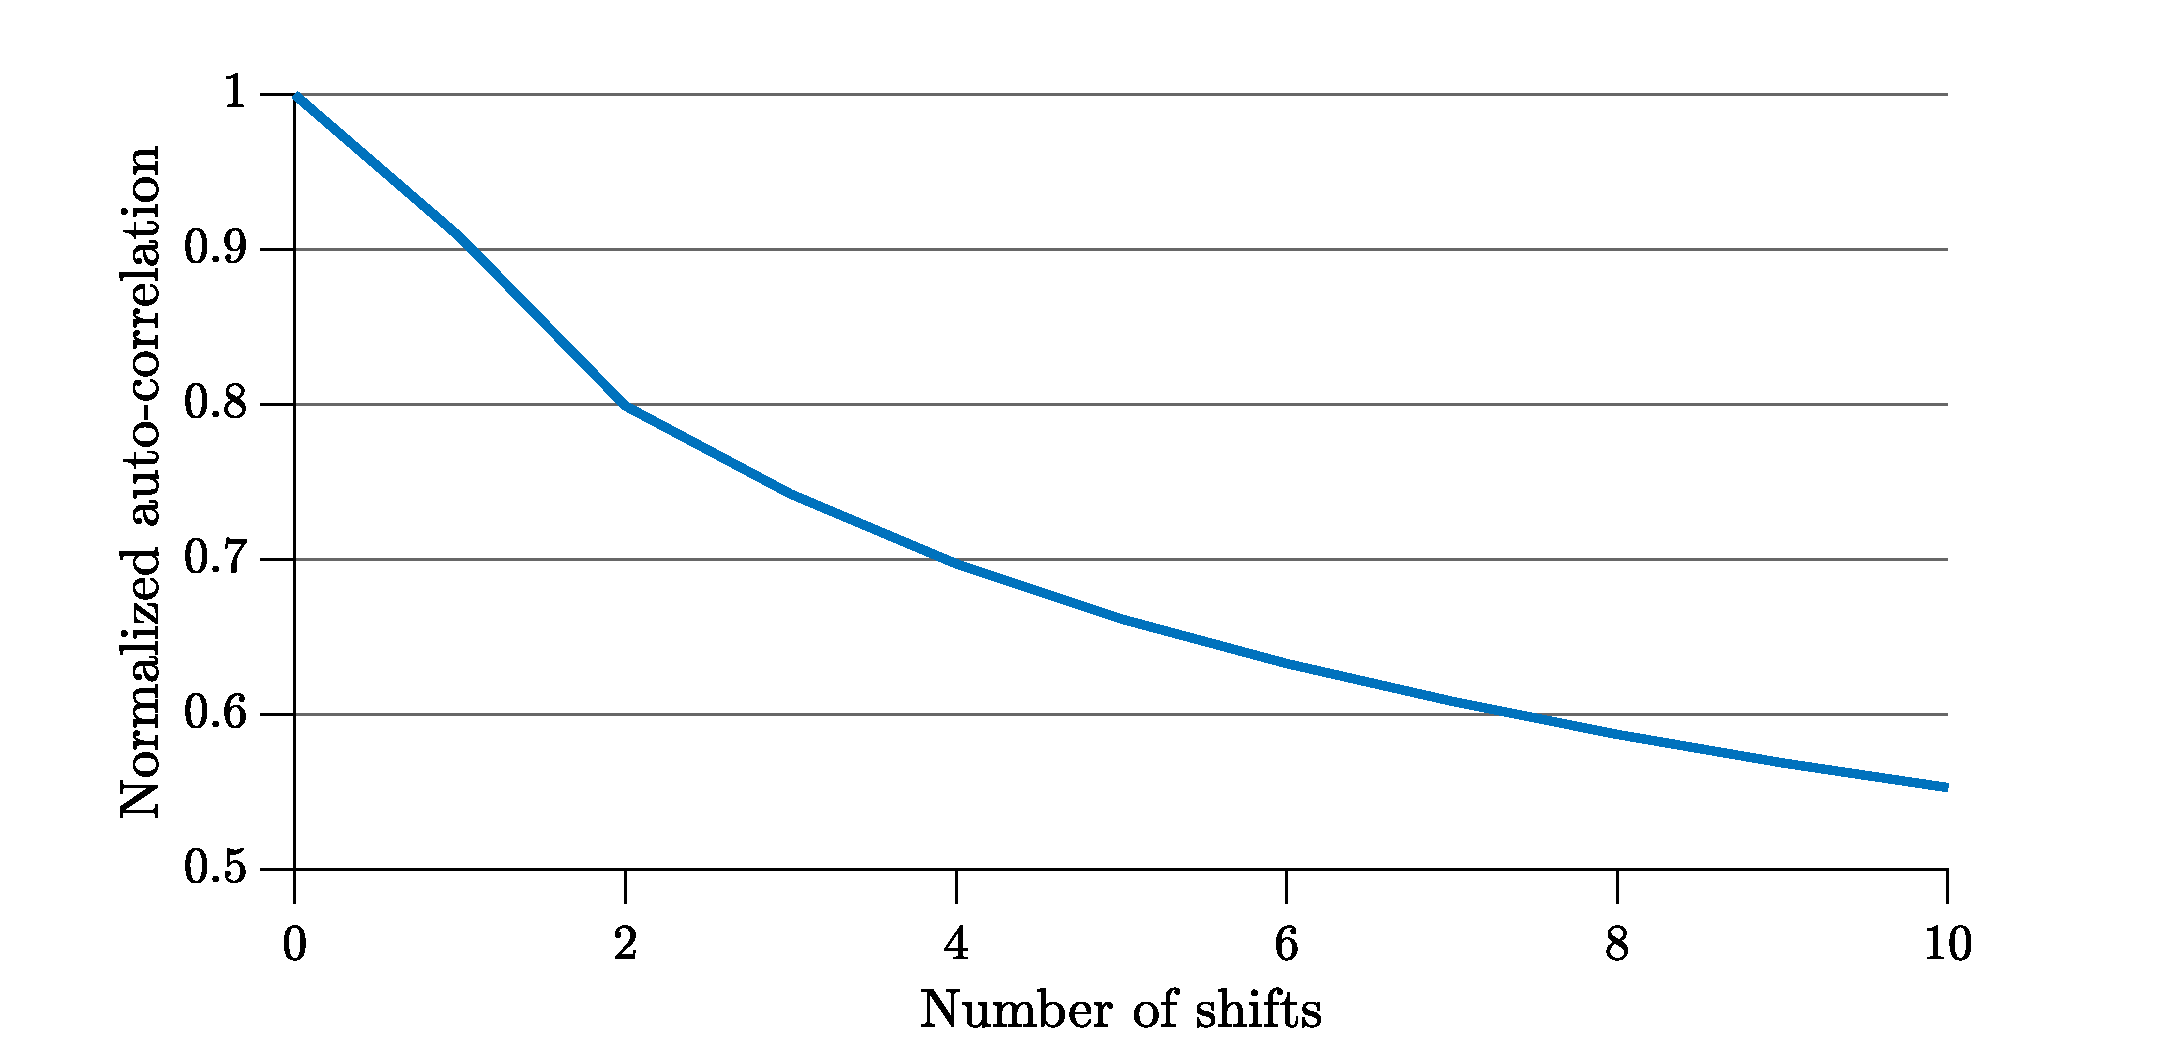
\includegraphics[width=\textwidth]{Sections/2AV1/Diagrams/intracorr.eps}
    \caption{Autocorrelation of image \ref{subfig:noiseOri}, with horizontal shifts}
    \label{fig:autocorr}
\end{figure}

As it is observable, for shorter shifts, the normalized autocorrelation is very close to 1, since most of the de-correlation comes for the mismatching edges. Although this relation varies depending on the image, it's safe to assume that it is very similar for the majority of the cases.

Such study gives a promising opportunity for compression, since it means that most pixels can be predicted from its neighbors. This aspect as lead to what now is known as \emph{differential} or \emph{predictive} coding.

On a video compression system, the spatial redundancy is considered in the \emph{intra-prediction} block, which calculates pixels, or pixel blocks, through its surrounds.

%%%%%%%%%%%%%%%%%%%
\subsubsection{Temporal Redundancy}

As expected, a series of consecutive frames, on the same subject, tend to be very similar between each other, especially if considered the $30$ or $60 fps$ desired nowadays. 

Making a similar analysis to what was made in section \ref{sssec:spatred}, a series of frames of the \emph{Stefan} sequence \cite{YUVSequences} was considered, and the cross correlation between the first and the following nine was calculated, giving origin to the graph in figure \ref{fig:crosscorr}.

\begin{figure}[h]
    \centering
    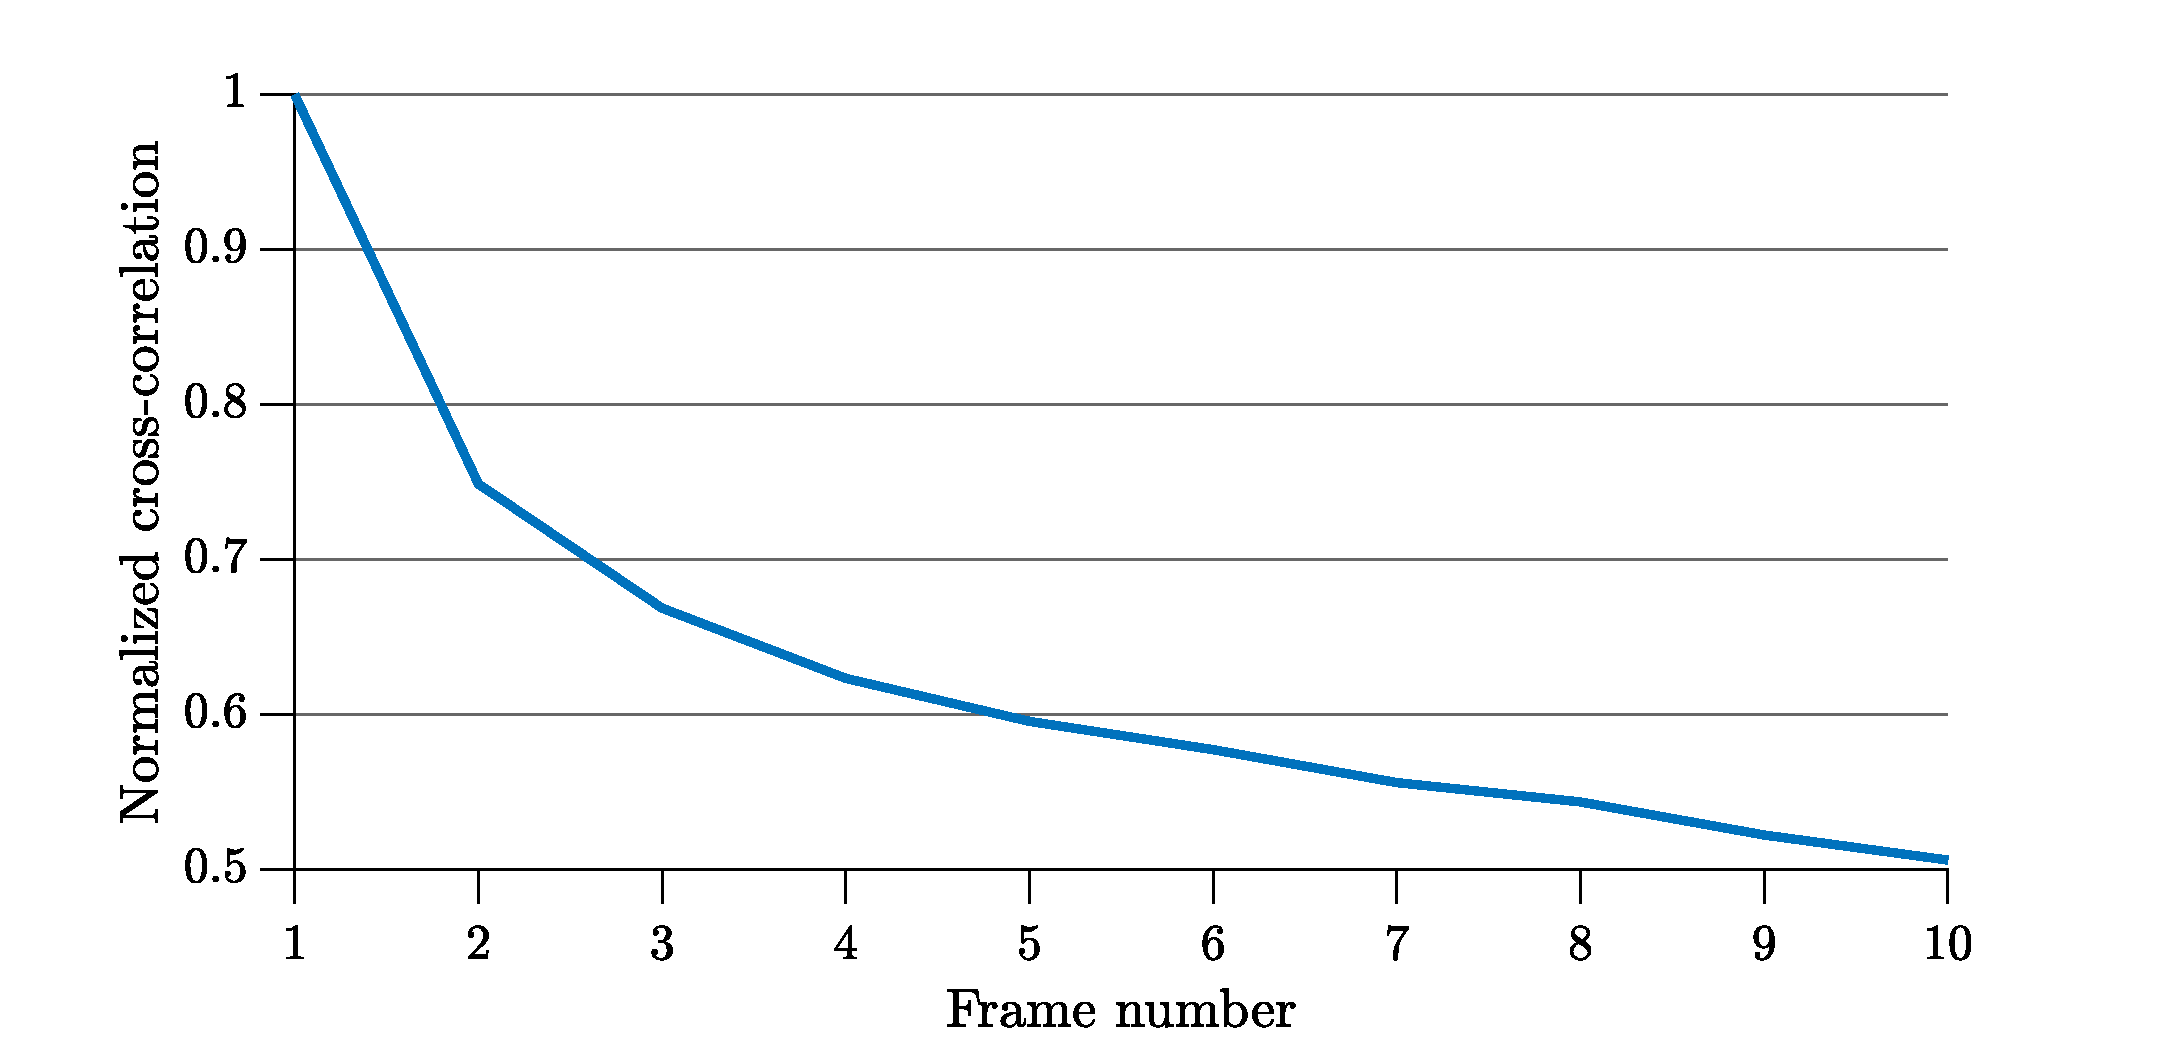
\includegraphics[width=\textwidth]{Sections/2AV1/Diagrams/intercorr.eps}
    \caption{Cross-correlation between the first and following nine frames of the \emph{Stefan} sequence}
    \label{fig:crosscorr}
\end{figure}

Similarly to what happened in the previous example, the cross correlation between consecutive frames is very high. Even though for faster moving scenes this relation might not be as pronounced, its application on video coding greatly contributes to the compression verified in the latest codecs. 

The codec takes advantage of this redundancy in the \emph{inter-prediction} stage, which is composed by the \emph{Motion Estimation} (MC) and \emph{Motion Compensation} (ME) blocks. On this stage, blocks of pixels in nearby frames are analyzed for movement, predicting its position for following frames.

%%%%%%%%%%%%%%%%%%%
\subsubsection{Psychovisual Redundancy}

From the redundancies presented in section \ref{ssec:hvs}, video codecs implement compression measures in various stages.

The first measure is the \emph{chroma subsampling}, which takes advantage of the lower perception to color, discarding some of the \emph{chroma} samples, depending on the subsampling chosen.

Typically, a pixel value is represented in one luminance and two chrominance values, on the \emph{YCbCr} color space. The subsampling is defined in through the relation of luminance to chroma samples, being the most common the 4:4:4, 4:2:2 and 4:2:0 standards, represented in figure \ref{fig:subsample}. In the first one, no chroma samples are discarded, which means that for each 4 luminance (\emph{Y}) samples, there are 4 \emph{Cb} and 4 \emph{Cr} samples. Correspondingly, in the second standard, for each 4 Y samples, only 2 of each color components are maintained. The last example, although its misleading term, means that only 1 of each 4 chroma samples are kept.

\begin{figure}[h]
    \centering 
        \begin{subfigure}[c]{\textwidth}
            \centering
            \input{Sections/2AV1/Diagrams/sub444.tex}
            \caption{4:4:4}
            \label{subfig:444}
        \end{subfigure}
        \begin{subfigure}[c]{\textwidth}
            \centering
            \begin{tikzpicture}[scale=0.45]    
    \coordinate (ycenter) at (2,3);
    \node[align=center] at (ycenter.north) {\textbf{Y}};
    \fill[gray!40] (0,0) rectangle (1,1);
    \fill[gray!70] (1,0) rectangle (2,1);
    \fill[gray!40] (2,0) rectangle (3,1);
    \fill[gray!70] (3,0) rectangle (4,1);
    \fill[gray!70] (0,1) rectangle (1,2);
    \fill[gray!40] (1,1) rectangle (2,2);
    \fill[gray!70] (2,1) rectangle (3,2);
    \fill[gray!40] (3,1) rectangle (4,2); 
    
    \coordinate (ccenter) at (7,3);
    \node[align=center] at (ccenter.north) {\textbf{Cb/Cr}};
    \fill[green] (5,0) rectangle (6,1);
    \fill[green] (6,0) rectangle (7,1);
    \fill[cyan] (7,0) rectangle (8,1);
    \fill[cyan] (8,0) rectangle (9,1);
    \fill[blue] (5,1) rectangle (6,2);
    \fill[blue] (6,1) rectangle (7,2);
    \fill[pink] (7,1) rectangle (8,2);
    \fill[pink] (8,1) rectangle (9,2);

\end{tikzpicture}
            \caption{4:2:2}
            \label{subfig:422}
        \end{subfigure}
        \begin{subfigure}[c]{\textwidth}
            \centering
            \input{Sections/2AV1/Diagrams/sub420.tex}
            \caption{4:2:0}
            \label{subfig:420}
        \end{subfigure}
       \caption{Representation of chroma subsampling}
    \label{fig:subsample}
\end{figure}

From the reduced sensitivity to details (or areas with high spatial frequency), the compression is explored in the \emph{Transform} (T) and \emph{Quantization} (Q) blocks. In the first stage, blocks of pixels are evaluated in their frequency components. These are then evaluated in the second stage, where the least significant ones get discarded. In the decoder, the image is reconstructed with the maintained coefficients, without much impact to the image quality. This process is further explained throughout the work.

On the Quantization block, some work was also developed to account for \emph{Weber's law}, where the quantization depends on the average luminance value of the block. This concept was first introduced in \cite{watsonEfficiencyModelHuman1988}, and since then experimented in various codecs, such as HEVC \cite{rouisPerceptualVideoContent2018}.

%%%%%%%%%%%%%%%%%%%
\subsubsection{Coding Redundancy}

Coding redundancy is directed to the method of representing information in the digital domain, i.e., the bits themselves, and how they are organized.

It is known that symbol probability plays a major role in information compression, across a wide variety of branches, and video is no exception. Taking this into account, codecs take advantage of coding redundancy in the \emph{Entropy Encoder} stage.

%%%%%%%%%%%%%%%%%%%%%%%%%%%%%%%%%%%%%%%
\subsection{Basic Video Compression/Decompression System}

From the basic principles of the previously mentioned blocks, it is possible to integrate them into two complete compression --- \emph{Encoder} --- and decompression --- \emph{Decoder} --- modules.

%%%%%%%%%%%%%%%%%%%
\subsubsection{Encoder Model} \label{ssse:encmod}

The encoder's objective is to compress a video sequence, turning it into a readable \emph{encoded bitstream}. To do this, the previously presented strategies get implemented on a system based on the schematic of figure \ref{fig:basicenc}.

\begin{figure}[!htbp]
    \centering
    \begin{tikzpicture}[%
    >=triangle 60,              % Nice arrows; your taste may be different
    start chain=going right,    % General flow is top-to-bottom
    node distance=2.5cm,          % Global setup of box spacing
    every join/.style={norm},   % Default linetype for connecting boxes
    ]

\tikzset{
    base/.style={draw, on chain, on grid, align=center},
    proc/.style={base, rectangle, text width=1.6cm, fill=black!15, minimum height=1.5cm, minimum width=1.5cm,font={\bfseries}},    
    frame/.style={base, minimum height=1.5cm, minimum width=2cm, fill=blue!10, thick},
    sub/.style={base, circle, inner sep=0pt, radius=0.4cm, fill=black!10, minimum height=3.5ex, font={\bfseries}},
    spot/.style={circle, inner sep=0pt, radius=0.4cm, minimum height=2mm, draw},
    edge rectangle/.style={ to path={ rectangle (\tikztotarget)}},
    % coord node style is used for placing corners of connecting lines
    coord/.style={coordinate, on chain, on grid, node distance=6mm and 40mm},
    % Arrows 
    fforw/.style={->, thick},
    fback/.style={->, thick, red!75!black},
    aref/.style={<->, dashed, black!50},
    % -------------------------------------------------
    % Connector line styles for different parts of the diagram
    cascaded/.style = {%
    general shadow = {%
      shadow scale = 1,
      shadow xshift = -1ex,
      shadow yshift = 1ex,
      draw,
      thick,
      fill = blue!40},
    general shadow = {%
      shadow scale = 1,
      shadow xshift = -.5ex,
      shadow yshift = .5ex,
      draw,
      thick,
      fill =blue!40},
    fill = blue!40, 
    draw,
    thick,
    minimum width = 2cm,
    minimum height = 1.5cm},
    base
}    

%% Top row
\node [frame] (inframe) {Input\\Frame};
    \node [coord] (ni1) {};    
    \node [coord, right=2mm of inframe.east] (ni2) {};
\node [sub, right=2cm of ni1] (sub) {-};
    \draw [fforw] (inframe) -- (sub);
\node [proc] (T) {T};
    \draw [fforw] (sub) -- (T);
\node [proc] (Q) {Q};
    \draw [fforw] (T) -- (Q);
\coordinate (rq) at ($(Q.east)+(4mm,0)$);
\node [proc, right=1cm of Q.east] (EC) {Entropy\\Coding};
    \draw [fforw] (Q) -- (EC);
\coordinate (out) at ($(EC.east)+(4mm,0)$);
%\path (EC) to node [yshift=-1em] {Encoded\\Bitstream} (out);
    \draw [fforw] (EC) -- (out);

%% Reference
\node [cascaded, below=5cm of inframe] (ref) {Reference\\Frames};

%% Intra
\node [proc, below=1.5cm of ni1] (intra) {Intra\\Coding};
    \coordinate (ni3) at (ni2 |- intra);    
    \draw [fforw] (ni3) -- (intra);

%% Inter    
\node [proc,right=of ref] (inter) {Inter\\Coding};
    \node [coord, below=4.5cm of ni2] (ni4) {};
    \draw [fforw] (ni2) -- (ni4) |- ($(inter.west)+(0,5mm)$);
    \draw [fforw] ($(ref.east)+(0,-5mm)$) -- ($(inter.west)+(0,-5mm)$);

%% Selector
\coordinate (rintra) at ($(intra.east)+(5mm,0)$);
\node [spot, below=1cm of rintra, fill=black] (sintra) {};
    \draw [thick] (intra.east) -- (rintra) |- (sintra.north);

\coordinate (rinter) at ($(inter.east)+(5mm,0)$);
\node [spot, above=1cm of rinter, fill=black] (sinter) {};
    \draw [thick] (inter.east) -- (rinter) |- (sinter.south);

\path (sintra) -- (sinter) coordinate [midway] (intraintermid);
\node [spot, at=(sub |- intraintermid)] (sel) {};
\draw [dashed] ($(sel)+(-2mm,3.3mm)$) arc (140:220:5mm);
    \draw [fforw] (sel) -- (sintra);
    \draw [fforw] (sel) -- (sub);

%% Lower Row    
\node [sub, below=3.7cm of sel] (add) {+};
    \draw [fback] (sel) -- (add);
\node [proc] (T1) {$\mathbf{T^{-1}}$};
    \draw [fback] (T1) -- (add);
\node [proc] (Q1) {$\mathbf{Q^{-1}}$};
    \draw [fback] (Q1) -- (T1);
\coordinate (rq1) at ($(Q1.east)+(4mm,0)$);
    \draw [fback] (rq) -- (rq1) |- (Q1);
\node [frame, below=7.4cm of inframe] (recframe) {Reconstructed\\Frame};
    \draw [fback] (add) -- (recframe);

%% Control
\path (inframe.west) -- (EC.east) node[midway] (mid) {};
\node [proc, text width=8cm, fill=black!40, above=2cm of mid, rounded corners, ] (control) {Control Unit};
    \draw [aref] (T) -- (T.north |- control.south);
    \draw [aref] (Q) -- (Q.north |- control.south);
\coordinate (aboveec) at (EC |- control);
    \draw [aref] (EC) -- (aboveec) |- (control);
    \draw [aref] (Q1.north) -- ++(0,5mm) |- ($(Q1.north west)+(-4mm,5mm)$) coordinate (y) |- (y |- control.south);
    \draw [aref] (T1.north) -- ++(0,5mm) |- ($(T1.north west)+(-4mm,5mm)$) coordinate (y) |- (y |- control.south);
    \draw [aref] (intra.north) -- (intra |- control.south);
    \draw [aref] (inter.south) -- ++(0,-3.2mm) |- ($(inter.south east)+(20mm,-3.2mm)$) coordinate (y) |- (y |- control.south);
\end{tikzpicture}
    \caption{Simplified Basic Encoder Model}
    \label{fig:basicenc}
\end{figure}

The encoding process starts on the \emph{Input Frame}, which can be of two types. \emph{I Frames} are encoded using only the information present in themselves, i.e., using only \emph{Intra Prediction/Coding}, while \emph{P Frames} may use predictive coding from previously encoded frames \footnote{Most video codecs allow that the encoding sequence isn't the same as the temporal sequence. This allows to reference frames displayed next to the one being encoded.}.

The input gets split into blocks, which get fed into the two main blocks of a video encoder: the \emph{Intra} and \emph{Inter} Prediction blocks.

The \emph{Intra Coding} block, as mentioned previously, deals with the spatial redundancy, by predicting the current block from the pixels above and to the left of its upper and left edges. The prediction may be done with various algorithms, ranging from calculating the average from the reference pixels, to replicating these according to a certain direction. One such example is presented in figure \ref{fig:intraex}, where pixels B through H get spread across a $4\times 4$ block, diagonally.

\begin{figure}[!htbp]
    \centering
    \begin{tikzpicture}[scale=0.7,>=triangle 60]
\tikzset{
    a/.style={->},
}    
    \draw [fill=lightgray] (0,0) rectangle (1,5);
    \draw [fill=lightgray] (1,4) rectangle (9,5);
    \draw[step=1cm,black,very thin] (0,0) grid (5,5);
    \draw[step=1cm,black,very thin] (5,4) grid (9,5);

    \node at (1.5,4.5) {A};
    \node at (2.5,4.5) {B};
    \node at (3.5,4.5) {C};
    \node at (4.5,4.5) {D};
    \node at (5.5,4.5) {E};
    \node at (6.5,4.5) {F};
    \node at (7.5,4.5) {G};
    \node at (8.5,4.5) {H};

    \node at (0.5,4.5) {I};
    \node at (0.5,3.5) {J};
    \node at (0.5,2.5) {K};
    \node at (0.5,1.5) {L};
    \node at (0.5,0.5) {M};

    \draw [a] (8,4) --(4,0);
    \draw [a] (7,4) --(3,0);
    \draw [a] (6,4) --(2,0);
    \draw [a] (5,4) --(1,0);
    \draw [a] (4,4) --(1,1);
    \draw [a] (3,4) --(1,2);
    \draw [a] (2,4) --(1,3);
\end{tikzpicture}
    \caption{Directional Intra-prediction example}
    \label{fig:intraex}
\end{figure}

Into the \emph{Inter Coding} block, go two inputs. The currently encoding block, as well as a bank of previously encoded frames, named \emph{Reference Frames}. Firstly, the frames inside the buffer get searched for blocks resembling the former input. Once found, this process generates a \emph{motion vector}, corresponding to the difference between the position of the block found in the reference frame, and the position of the currently encoding block, as shown in figure \ref{fig:interex}.

\begin{figure}[!htbp]
    \centering
    \begin{tikzpicture}[scale=.7,every node/.style={minimum size=1cm},on grid,>=triangle 60]
		
    %slanting: production of a set of n 'laminae' to be piled up. N=number of grids.
    \begin{scope}[
            yshift=-83,every node/.append style={
            yslant=0.5,xslant=-1},yslant=0.5,xslant=-1
            ]
        % opacity to prevent graphical interference
        \fill[white,fill opacity=0.9] (0,0) rectangle (5,5);
        \draw[blue!40!black,very thick] (0,0) rectangle (5,5);%marking borders
        \filldraw[blue!30] (0.5,0.5) rectangle (1.5,1.5);
        \draw[gray, dashed] (0.5,1.5) -- (3.42,4.42);
        \draw[gray, dashed] (1.5,0.5) -- (4.42,3.42);
        \draw[gray, dashed] (0.5,0.5) -- (3.42,3.42);
        \draw[gray, dashed] (1.5,1.5) -- (4.42,4.42);
        %Idem as above, for the n-th grid:
    \end{scope}
    
    \begin{scope}[
    	    yshift=0,every node/.append style={
    	    yslant=0.5,xslant=-1},yslant=0.5,xslant=-1
            ]
        \fill[white,fill opacity=.9] (0,0) rectangle (5,5);
        \draw[black,very thick] (0,0) rectangle (5,5);

        \draw[blue!30] (0.5,0.5) rectangle (1.5,1.5);
        \filldraw[gray] (2.5,3) rectangle (3.5,4);

        \draw[->] (0.5,0.5) -- (2.5,3);
    \end{scope}

    \draw[-latex,thick](5.8,0)node[right]{Reference Frame}
    to[out=180,in=90] (3.4,-1);

    \draw[-latex,thick] (5.8,3) node[right]{Present Frame}
         to[out=180,in=90] (3.4,2);

    \draw[-latex,thick] (-5.5,2.2) node[left]{Motion Vector}
    to [out=0,in=180](-0.22,1.5);
\end{tikzpicture}
    \caption{Inter-prediction example}
    \label{fig:interex}
\end{figure}

In most codecs, the motion vector has a precision below one pixel. This means that the matching block, from the reference frame, may be interpolated from existing pixels. This process is named as \emph{sub-pixel interpolation}, which calculates virtual values between existing pixels. 

After the prediction stage, the chosen output between the two processes, i.e., the predicted block, gets subtracted by the current one, giving origin to the \emph{residue}. This corresponds to the pixel value differences between the original and predicted blocks. Lower \emph{residues} indicate more efficient prediction stages.

The next stage, the \emph{Forward Transform}, is the focus of this work. It takes the residue blocks, which may not be the same size of the prediction blocks, and evaluates them according to its spatial frequencies. Its output corresponds to a series of \emph{coefficients}, that are related to the similarity --- or \emph{correlation} --- between the input block and a series of \emph{basis images}. This process is further explained in chapter \ref{chap:trans}.

On the \emph{Quantization} stage, the coefficients calculated in \textbf{T} get scaled according to a \emph{Quantization Matrix}. This stage takes advantage of the eye's lower perception to high frequency details, and scales the higher frequency coefficients by a higher value, than the lower, more significant ones. In most of the transformed blocks, this leads that only a few low frequency components are maintained, while the others get nullified, since they are not relevant to the reconstruction of the image. Therefore, this stage is the the one that presents the higher loss, although the previously presented also introduce errors.

The wipe out of the least significant coefficients is particularly efficient when paired with the last stage before the output, the \emph{Entropy Encoder}. On this block, \textbf{Q}'s output block gets run sequentially via a \emph{zig-zag scan}, which first passes through the lower frequency coefficients, followed by the higher frequency ones. 

\begin{figure}[!htbp]
    \centering
    \begin{tikzpicture}[scale=0.7,>=triangle 60]
    \tikzset{
        a/.style={>->, thick},
    }    
        \draw[step=1cm,black,very thin] (0,0) grid (8,8);
    
        \draw [a] (0.5,7.5) -- (1.5,7.5) -- (0.5,6.5) -- (0.5,5.5) -- (2.5,7.5) -- (3.5,7.5) -- (0.5,4.5) -- (0.5,3.5) -- (4.5,7.5) -- (5.5,7.5) -- (0.5,2.5) -- (0.5,1.5) -- (6.5,7.5) -- (7.5,7.5) -- (0.5,0.5) -- (1.5,0.5) -- (7.5,6.5) -- (7.5,5.5) -- (2.5,0.5) -- (3.5,0.5) -- (7.5,4.5)  -- (7.5,3.5) -- (4.5,0.5)  -- (5.5,0.5) -- (7.5,2.5) -- (7.5,1.5)  -- (6.5,0.5)  -- (7.5,0.5);

        \draw [->, -latex] (3,8.5) -- node[above, font={\small}]{Horizontal Frequency ($u$)} (5,8.5);

        \draw [->, -latex] (-0.5,5) -- node[above, font={\small}, rotate=90]{Vertical Frequency ($v$)} (-0.5,3);
    \end{tikzpicture}
    \caption{Demonstration of Zig-Zag Scan}
    \label{fig:zigzag}
\end{figure}

In most of the cases, this causes that the non-zero coefficients get read first, followed by a sequence of zeros. Such sequence benefits heavily of being encoded with \gls{vlc}, such as \emph{Huffman Tree Codes} or \Gls{cabac}. Off all the processes, this is the one that doesn't introduce further distortion into the encoded sequence, which is the reason it doesn't get included in the \emph{feedback loop}.

The intent of this loop is to get an exact same copy of the frame reconstructed in the decoder. This reconstructed frame gets used as the reference for intra-prediction, or gets put into the reference frame buffer to be used in a later inter-prediction process. 

The output of the encoder is the quantized coefficients, as well as the necessary information to recreate the encoded blocks, such as the type of prediction used, the transformation \emph{kernel} [see p.\pageref{par:kernel}], quantization matrix, et al. These encoding parameters are the choices made by the \emph{Control Unit}, which although represented by a block in figure \ref{fig:basicenc}, may not be a local process, independent from all others. 

Since \emph{H.264}, most video codecs standardize the decoding process, specifically, the allowed tools for compressing the video, and how to use them. This means that the encoding process is widely adaptable to the compression objectives, as long as the final product is a bitstream following the norms set on the codec's standard \cite{AV1BitstreamDecoding}. Therefore, the definition of a \emph{Control Unit} is ambiguous in this context, since such unit can simply represent a set of parameters to be used throughout the encoding process\footnote{One such example would be \emph{lossless} compression modes, which use very a concise conditions on each stage, in order to get the least distortion.}, or an algorithm that can change between the different capabilities of the codec, in order to achieve an objective, such as a specific distortion rate, or not surpass a maximum bit rate. As expected, different objectives may lead to majorly different results, both in the output video, as well as in the used tools.

%%%%%%%%%%%%%%%%%%%
\subsubsection{Decoder Model}

As expected, the decoder (figure \ref{fig:basicdec}) does the backwards operation of the encoder on figure \ref{fig:basicenc}. It starts by analyzing the bitstream, separating the control information from the encoded and quantized coefficients.

\begin{figure}[!htbp]
    \centering
    \begin{tikzpicture}[%
    >=triangle 60,              % Nice arrows; your taste may be different
    start chain=going right,    % General flow is top-to-bottom
    node distance=2.5cm,          % Global setup of box spacing
    every join/.style={norm},   % Default linetype for connecting boxes
    ]

\tikzset{
    base/.style={draw, on chain, on grid, align=center},
    proc/.style={base, rectangle, text width=1.6cm, fill=black!15, minimum height=1.5cm, minimum width=1.5cm,font={\bfseries}},    
    frame/.style={base, minimum height=1.5cm, minimum width=2cm, fill=blue!10, thick},
    sub/.style={base, circle, inner sep=0pt, radius=0.4cm, fill=black!10, minimum height=3.5ex, font={\bfseries}},
    spot/.style={circle, inner sep=0pt, radius=0.4cm, minimum height=2mm, draw},
    edge rectangle/.style={ to path={ rectangle (\tikztotarget)}},
    % coord node style is used for placing corners of connecting lines
    coord/.style={coordinate, on chain, on grid, node distance=6mm and 40mm},
    % Arrows 
    fforw/.style={->, thick},
    fback/.style={->, thick, red!75!black},
    aref/.style={<->, dashed, black!50},
    % -------------------------------------------------
    % Connector line styles for different parts of the diagram
    cascaded/.style = {%
    general shadow = {%
      shadow scale = 1,
      shadow xshift = -1ex,
      shadow yshift = 1ex,
      draw,
      thick,
      fill = blue!40},
    general shadow = {%
      shadow scale = 1,
      shadow xshift = -.5ex,
      shadow yshift = .5ex,
      draw,
      thick,
      fill =blue!40},
    fill = blue!40, 
    draw,
    thick,
    minimum width = 2cm,
    minimum height = 1.5cm},
    base
}    

\node [coord] (ed) {};    
\node[proc, text width=2cm, right=4mm of ed] (ED) {Entropy\\Decoding};
    \draw [fforw] (ed) -- (ED.west);
\node [proc] (Q1) {$\mathbf{Q^{-1}}$};
    \draw [fforw] (ED) -- (Q1);
\node [proc] (T1) {$\mathbf{T^{-1}}$};
    \draw [fforw] (Q1) -- (T1);
\node [sub] (add) {+};
    \draw [fforw] (T1) -- (add);
\node [frame, right=5cm of add] (recframe) {Reconstructed\\Frame};
    \draw [fforw] (add) -- (recframe);

%% Inter
\node [cascaded, below=5cm of recframe] (ref) {Reference\\Frames};
\node [proc, left=of ref] (inter) {Inter\\Coding};
\draw [fforw] (ref) -- (inter);

%% Intra
\coordinate (lrec) at (inter |- recframe);
\node [proc, below=1.5cm of lrec] (intra) {Intra\\Coding};
    \draw [fforw] (intra |- recframe) -- (intra.north);

%% Selector
\coordinate (lintra) at ($(intra.west)+(-5mm,0)$);
\node [spot, below=1cm of lintra, fill=black] (sintra) {};
    \draw [thick] (intra.west) -- (lintra) |- (sintra.north);

\coordinate (linter) at ($(inter.west)+(-5mm,0)$);
\node [spot, above=1cm of linter, fill=black] (sinter) {};
    \draw [thick] (inter.west) -- (linter) |- (sinter.south);

\path (sintra) -- (sinter) coordinate [midway] (intraintermid);
\node [spot, at=(add |- intraintermid)] (sel) {};
\draw [dashed] ($(sel)+(4mm,-3.3mm)$) arc (-40:40:5mm);
    \draw [fforw] (sintra) -- (sel);
    \draw [fforw] (sel) -- (add);

%% Control
\path (ED.west) -- (recframe.east) node[midway] (mid) {};
\node [proc, text width=8cm, fill=black!40, above=2cm of mid, rounded corners, ] (control) {Control Unit};
    \draw [aref] (T1) -- (T1.north |- control.south);
    \draw [aref] (Q1) -- (Q1.north |- control.south);
\coordinate (aboved) at (ED |- control);
    \draw [aref] (ED) -- (aboved) |- (control);
    \draw [aref] (intra.120) -- (intra.120 |- control.south);
    \draw [aref] (inter.south) -- ++(0,-3.2mm) coordinate (y) |- (control.south |- y) |- (control.south);
    \draw [aref] (sel.west) -- ++(-6mm,0) coordinate (y) |- (y |- control.south);

%% Legend
\node [below=5cm of ED, font={\tiny}] (lc) {Control\\Signal};
    \draw [aref] ($(lc.west)+(-6mm,0)$) -- +(5mm,0);
\node [above=7mm of lc, font={\tiny}] (lf) {Forward\\Path};
    \draw [fforw] ($(lc.west)+(-6mm,7mm)$) -- +(5mm,0); 
\draw[thick] ($(lc.south west)+(-9mm,-2mm)$) rectangle ($(lf.north east)+(2mm,2mm)$);

\end{tikzpicture}
    \caption{Simplified Basic Decoder Model}
    \label{fig:basicdec}
\end{figure}

Having the encoding choices performed by the encoder, the decoder returns the \emph{coding redundancy} to the quantized coefficients, on the \emph{Entropy Decoding} stage. This corresponds to a translation from the varying length code used in codification, back into the raw coefficients.

The \emph{Inverse Quantization} rescales the maintained coefficients, resulting from the previous \emph{Quantization} stage. With this, it is meant that the same quantization matrix used when dividing the transformed coefficients, in the encoder, is now multiplied by the quantized parameters. It must be kept that this operation does not output an exact copy of the transformation coefficients, as a lot of information is permanently lost in \textbf{Q}. This process can be seen in figure \ref{fig:quant}.

\begin{figure}[!htbp]
    \centering
    \begin{tikzpicture}[scale=0.5,>=triangle 60]
    \def\intrans{
        {19, -1, 0, 1, -1, 8, 3, -3, -3, -2, 1, -7, -3, -4, 8, 0}
    }
    \tikzset{
        a/.style={>->, thick},
    }    
    \node (inres) [inner sep=0pt, draw, label={[align=center, font={\small\bfseries}]above:Input\\Residue}, fit={(0,0) (4,4)}] {};
        \draw[step=1cm,black,very thin, inner sep=0pt] (0,0) grid (4,4);   
            \node at (0.5, 0.5) {6};
            \node at (0.5, 1.5) {-3};
            \node at (0.5, 2.5) {5};
            \node at (0.5, 3.5) {6};
            \node at (1.5, 0.5) {0};
            \node at (1.5, 1.5) {9};
            \node at (1.5, 2.5) {8};
            \node at (1.5, 3.5) {8};
            \node at (2.5, 0.5) {8};
            \node at (2.5, 1.5) {7};
            \node at (2.5, 2.5) {-2};
            \node at (2.5, 3.5) {5};
            \node at (3.5, 0.5) {7};
            \node at (3.5, 1.5) {7};
            \node at (3.5, 2.5) {6};
            \node at (3.5, 3.5) {-1};
    
    \node [inner sep=0pt, draw, right=1 of inres, label={[align=center, font={\small\bfseries}]above:Transformed\\Coefficients}, fit={(5,0) (9,4)}] (intrans) {};
        \draw[step=1cm,black,very thin, inner sep=0pt] (intrans.south west) grid (intrans.north east);   
                    \node at ($(intrans.south west)+(0.5,0.5)$) {1};
                    \node at ($(intrans.south west)+(0.5,1.5)$) {0};
                    \node at ($(intrans.south west)+(0.5,2.5)$) {-1};
                    \node at ($(intrans.south west)+(0.5,3.5)$) {19};
                    \node at ($(intrans.south west)+(1.5,0.5)$) {-3};
                    \node at ($(intrans.south west)+(1.5,1.5)$) {3};
                    \node at ($(intrans.south west)+(1.5,2.5)$) {8};
                    \node at ($(intrans.south west)+(1.5,3.5)$) {-1};
                    \node at ($(intrans.south west)+(2.5,0.5)$) {-7};
                    \node at ($(intrans.south west)+(2.5,1.5)$) {1};
                    \node at ($(intrans.south west)+(2.5,2.5)$) {-2};
                    \node at ($(intrans.south west)+(2.5,3.5)$) {-3};
                    \node at ($(intrans.south west)+(3.5,0.5)$) {0};
                    \node at ($(intrans.south west)+(3.5,1.5)$) {8};
                    \node at ($(intrans.south west)+(3.5,2.5)$) {-4};
                    \node at ($(intrans.south west)+(3.5,3.5)$) {-3};

    \node [draw, circle, fill=lightgray, right=1 of intrans, minimum height=0.5, font={\bfseries}] (div) {$\div$};

    \node [inner sep=0pt, draw, below right=3 and 3 of div, label={[align=center, font={\small\bfseries}]above:Quantized\\Coefficients}, fit={(11,0) (15,4)}] (inq) {};
        \draw[step=1cm,black,very thin, inner sep=0pt] (inq.south west) grid (inq.north east);   
                \node at ($(inq.south west)+(0.5,0.5)$) {0};
                \node at ($(inq.south west)+(0.5,1.5)$) {0};
                \node at ($(inq.south west)+(0.5,2.5)$) {-1};
                \node at ($(inq.south west)+(0.5,3.5)$) {19};
                \node at ($(inq.south west)+(1.5,0.5)$) {-1};
                \node at ($(inq.south west)+(1.5,1.5)$) {1};
                \node at ($(inq.south west)+(1.5,2.5)$) {3};
                \node at ($(inq.south west)+(1.5,3.5)$) {-1};
                \node at ($(inq.south west)+(2.5,0.5)$) {-1};
                \node at ($(inq.south west)+(2.5,1.5)$) {0};
                \node at ($(inq.south west)+(2.5,2.5)$) {0};
                \node at ($(inq.south west)+(2.5,3.5)$) {-1};
                \node at ($(inq.south west)+(3.5,0.5)$) {0};
                \node at ($(inq.south west)+(3.5,1.5)$) {1};
                \node at ($(inq.south west)+(3.5,2.5)$) {-1};
                \node at ($(inq.south west)+(3.5,3.5)$) {-1};

    \node [inner sep=0pt, draw, below left=3 and 2 of div, label={[align=center, font={\small\bfseries}]above:Quantization\\Matrix}, fit={(11,0) (15,4)}] (qm) {};
        \draw[step=1cm,black,very thin, inner sep=0pt] (qm.south west) grid (qm.north east);   
            \node at ($(qm.south west)+(0.5,0.5)$) {4};
            \node at ($(qm.south west)+(0.5,1.5)$) {3};
            \node at ($(qm.south west)+(0.5,2.5)$) {2};
            \node at ($(qm.south west)+(0.5,3.5)$) {1};
            \node at ($(qm.south west)+(1.5,0.5)$) {5};
            \node at ($(qm.south west)+(1.5,1.5)$) {4};
            \node at ($(qm.south west)+(1.5,2.5)$) {3};
            \node at ($(qm.south west)+(1.5,3.5)$) {2};
            \node at ($(qm.south west)+(2.5,0.5)$) {7};
            \node at ($(qm.south west)+(2.5,1.5)$) {6};
            \node at ($(qm.south west)+(2.5,2.5)$) {6};
            \node at ($(qm.south west)+(2.5,3.5)$) {3};
            \node at ($(qm.south west)+(3.5,0.5)$) {9};
            \node at ($(qm.south west)+(3.5,1.5)$) {8};
            \node at ($(qm.south west)+(3.5,2.5)$) {7};
            \node at ($(qm.south west)+(3.5,3.5)$) {6};
    
    \node [inner sep=0pt, draw, below left=6 and 2 of div, label={[align=center, font={\small\bfseries}]above:Restored\\Coefficients}, fit={(11,0) (15,4)}] (outq) {};
        \draw[step=1cm,black,very thin, inner sep=0pt] (outq.south west) grid (outq.north east);   
            \node at ($(outq.south west)+(0.5,0.5)$) {0};
            \node at ($(outq.south west)+(0.5,1.5)$) {0};
            \node at ($(outq.south west)+(0.5,2.5)$) {-2};
            \node at ($(outq.south west)+(0.5,3.5)$) {19};
            \node at ($(outq.south west)+(1.5,0.5)$) {-5};
            \node at ($(outq.south west)+(1.5,1.5)$) {4};
            \node at ($(outq.south west)+(1.5,2.5)$) {9};
            \node at ($(outq.south west)+(1.5,3.5)$) {-2};
            \node at ($(outq.south west)+(2.5,0.5)$) {-7};
            \node at ($(outq.south west)+(2.5,1.5)$) {0};
            \node at ($(outq.south west)+(2.5,2.5)$) {0};
            \node at ($(outq.south west)+(2.5,3.5)$) {-3};
            \node at ($(outq.south west)+(3.5,0.5)$) {0};
            \node at ($(outq.south west)+(3.5,1.5)$) {8};
            \node at ($(outq.south west)+(3.5,2.5)$) {-7};
            \node at ($(outq.south west)+(3.5,3.5)$) {-6};

    \node [draw, circle, fill=lightgray, right=of outq, minimum height=0.5, font={\bfseries}] (mul) {$\times$};

    \node [inner sep=0pt, draw, left=of outq, label={[align=center, font={\small\bfseries}]above:Restored\\Residue}, fit={(2,-12) (6,-8)}] (outt) {};
    \draw[step=1cm,black,very thin, inner sep=0pt] (outt.south west) grid (outt.north east);   
        \node at ($(outt.south west)+(0.5,0.5)$) {5};
        \node at ($(outt.south west)+(0.5,1.5)$) {-5};
        \node at ($(outt.south west)+(0.5,2.5)$) {5};
        \node at ($(outt.south west)+(0.5,3.5)$) {5};
        \node at ($(outt.south west)+(1.5,0.5)$) {1};
        \node at ($(outt.south west)+(1.5,1.5)$) {9};
        \node at ($(outt.south west)+(1.5,2.5)$) {9};
        \node at ($(outt.south west)+(1.5,3.5)$) {10};
        \node at ($(outt.south west)+(2.5,0.5)$) {10};
        \node at ($(outt.south west)+(2.5,1.5)$) {7};
        \node at ($(outt.south west)+(2.5,2.5)$) {-4};
        \node at ($(outt.south west)+(2.5,3.5)$) {2};
        \node at ($(outt.south west)+(3.5,0.5)$) {6};
        \node at ($(outt.south west)+(3.5,1.5)$) {9};
        \node at ($(outt.south west)+(3.5,2.5)$) {7};
        \node at ($(outt.south west)+(3.5,3.5)$) {0};


    \draw [->, very thick, gray] (inres.east)+(0.5,0) -- node[above]{\textbf{T}} +(2.5,0);
    \draw [->] (intrans.east)+(0.5,0) -- +(1.5,0);
    \draw [->] ($(qm.east)+(0.5,0)$) -- (div |- qm) |- ($(div.south)+(0,-0.5)$);
    \draw [->] ($(qm.east)+(0.5,0)$) -- (div |- qm) -| ($(mul.north)+(0,0.5)$);
    \draw [->, very thick, gray] ($(div)+(-45:1)$) -- node[above,sloped,near start]{\textbf{Q}} ($(inq.west)+(-0.2,0.4)$);
    \draw [->] ($(inq.west)+(-0.2,-0.4)$) -- ($(mul)+(45:1)$);
    \draw [->, very thick, gray] (mul.west)+(-0.5,0) -- node[above,sloped,yshift=3]{$\mathbf{Q^{-1}}$} +(-1.5,0);
    \draw [->, very thick, gray] (outq.west)+(-0.5,0) -- node[above,sloped,yshift=3]{$\mathbf{T^{-1}}$} +(-2.5,0);
\end{tikzpicture}
    \caption{Processing of $\protect 4\times 4$ residue block from \emph{transformation} to restoring} 
    \label{fig:quant}
\end{figure}

As can also be seen in this figure, the \emph{Inverse Transform} converts the coefficients back into spatial coordinates, therefore getting the restored residue. To obtain the final approximation of the block being decoded, this residue must be added to the same predicted block from the encoder. To do so, the \emph{Intra} or \emph{Inter Prediction} stages act according to the choices made in the encoding process, as to regenerate this block.

In the decoder, the \emph{Control Unit} represents the process that organizes the different stages, according to the choices done in the encoding stage.

\nocite{agostiniDesenvolvimentoArquiteturasAlto2007}

%%%%%%%%%%%%%%%%%%%%%%%%%%%%%%%%%%%%%%%%%%%%%%%%%%%%%%%%%%%%%%%%%%%%%%%%%%%%%%
\section{AV1}

Being the focus of this work, in the following sections, \emph{AV1} is presented on its most relevant aspects, starting with its development process.

%%%%%%%%%%%%%%%%%%%%%%%%%%%%%%%%%%%%%%%
\subsection{History and Development}

\nocite{debarghamukherjeeAllThingsRTC2019Opening2019}

The development of this codec started as a need to improve the bandwidth reduction of \emph{VP9}. Therefore, the presentation of \emph{AV1} starts by explaining the guidelines of its predecessor.

\emph{VP9} started with project \emph{Webm}, created by \emph{On2}, which got acquired by \emph{Google} in 2010. This project had the objective of developing the first\footnote{VP8 got openly released after the acquisition of the company, after closing the development process.} open-source, royalty-free video codec. This got support from major video content producers, such as \emph{YouTube}, \emph{Netflix} and \emph{Twitch}, since it represented large savings in licensing payments, from the use of MPEG's standards, which got aggravated from the difficult patenting terms of \emph{HEVC} \cite{streamingmediaHEVCAdvancePatent2015}. After release in 2013, \emph{VP9} got adopted as \emph{YouTube}'s default video codec for video's above \emph{420p}, as well as other web-video consumption services, including \emph{Facebook}.

In 2014, \emph{Google} started working on the next generation of open-source video codecs, \emph{VP10}. However, due to the large interest from other companies which already used the previous standard, in 2015, the \emph{Alliance for Open Media} was created, and the the development made for this standard got inserted into \emph{AV1}. Alongside \emph{Google}, twelve other companies started \emph{AOM}, including two which also had open video encoder projects, which also majorly contributed to the fast development of \emph{AV1}: \emph{Cisco}'s \emph{Thor} and \emph{Mozilla}'s \emph{Daala}. As the time of writing, 42 companies are official members of \emph{AOM}, englobing a wide range of markets, from video streaming services, to hardware producers.

\begin{figure}[!htbp]
    \centering
    \includegraphics[width=\textwidth]{Sections/2AV1/Diagrams/Images/AOM.png}
    \caption[\emph{Alliance for Open Media} current members]{\emph{Alliance for Open Media} current members \cite{aomediaHome}} 
    \label{fig:aom}
\end{figure}

By 2016, \emph{AV1} started, with the objective of reaching 30\% bitrate decrease, in comparison to \emph{VP9}. After the bitstream freeze in March 2018 and deployment of \emph{libaom} soon later, this first objective was fulfilled. However, the compression performance did not atone for the very high compression and decompression times of the reference software. This left a large margin for improvement, which quickly got explored with the development of other compression and decompression algorithms by the \emph{AOM} members, such as \emph{dav1d}, \emph{rav1e}, \emph{SVT-AV1},  among others. This parallel development gave origin to a competition among the corresponding teams, that benefited the adoption of the standard, since it brought a wide range of possibilities. 

With the improvements verified on both encoders and decoders, \emph{AV1} got progressively more adoption from the industry, getting support from most web browsers, as well as uploads of \emph{AV1} encoded videos to streaming platforms \cite{eggeLatestTechnicalBusiness2019}.

Besides the advances in software solutions, shortly after the bitstream freeze, IC development companies started to develop hardware solutions. The focus started by hardware decoders for implementation in mobile devices, but some encoder solutions also have been announced. Although some claims of throughput up to \emph{8k 60fps} have been made, third party performance tests still remain to be published \cite{AllegroDVTIntroduces2019,NGCodecAnnouncesAV1, shilovRealtekDemonstratesRTD2893, RealtekLaunchesWorldwide, SocionextImplementsAV12018}.

%%%%%%%%%%%%%%%%%%%%%%%%%%%%%%%%%%%%%%%
\subsection{Encoding Tools}

\nocite{chenOverviewCoreCoding2018}

Although the focus of this work revolves around the Transform stage, in this section, \emph{AV1} is presented on its most relevant aspects. Some analogies are also made with \emph{VP9}'s tools, as to justify the performance increases obtained with the most recent generation, as well as the complexity.

%%%%%%%%%%%%%%%%%%%
\subsubsection{Partitioning}

At the start of the encoding process, an input frame is divided into \emph{superblocks}. These constitute the starting point of the compression of an image.

These blocks may be of $128 \times 128$ pixels, or $64 \times 64$. However, doing operations with such sizes would add complexity, as well as it wouldn't prove to be efficient. Therefore, the \emph{superblock} can be partitioned into various \emph{prediction blocks}. These can range between $128 \times 128$ to $4 \times 4$, including rectangular blocks, with $2:1$ or $4:1$ ratios. The division of these blocks can be done recursive, where a square block divided into 4 square blocks can originate progressively smaller blocks, according to the schematic in figure \ref{fig:partitioning}.

\begin{figure}[!htbp]
    \centering
    \begin{tikzpicture}[scale=0.6, every node/.style={scale=0.6}, >=triangle 60]
    \tikzset{
        a/.style={->, thick},
        sq/.style={draw, rectangle, minimum width=2cm, minimum height=2cm, fill=lightgray, thick}
    }    
    
    \begin{scope}
        \node [sq] (center) {};

        \node at ($(center)+(0:5cm)$) [sq] (heck) {};
            \draw (heck.south west) rectangle (heck);
            \draw (heck.west) rectangle (heck.north);
            \draw (heck) rectangle (heck.south east);
            \draw (heck) rectangle (heck.north east);

            \draw [a] (center) -- (heck);
            \draw [a] ($(heck.west)+(0,-1mm)$) to [bend left=22] ($(center.east)+(0,-1mm)$);

        \node at ($(center)+(36:5cm)$) [sq] (heck) {};
            \draw (heck.south west) rectangle (heck);
            \draw (heck.west) rectangle (heck.north);
            \draw (heck.south) rectangle (heck.north east);

            \draw [a] (center) -- (heck);

        \node at ($(center)+(72:5cm)$) [sq] (heck) {};
            \draw (heck.south west) rectangle (heck.east);
            \draw (heck.west) rectangle (heck.north);
            \draw (heck) rectangle (heck.north east);

            \draw [a] (center) -- (heck);

        \node at ($(center)+(106:5cm)$) [sq] (heck) {};
            \draw (heck.south west) rectangle (heck);
            \draw (heck.south) rectangle (heck.east);
            \draw (heck.west) rectangle (heck.north east);

            \draw [a] (center) -- (heck);

        \node at ($(center)+(142:5cm)$) [sq] (heck) {};
            \draw (heck.south west) rectangle (heck.north);
            \draw (heck.south) rectangle (heck.east);
            \draw (heck) rectangle (heck.north east);        

            \draw [a] (center) -- (heck);

        \node at ($(center)+(178:5cm)$) [sq] (heck) {};
            \draw [sq] (heck) {};

            \draw [a] (center) -- (heck);

        \node at ($(center)+(214:5cm)$) [sq] (heck) {};
            \draw (heck.south west) rectangle (heck.east);
            \draw (heck.west) rectangle (heck.north east);

            \draw [a] (center) -- (heck);

        \node at ($(center)+(250:5cm)$) [sq] (heck) {};
            \draw (heck.south west) rectangle (heck.north);
            \draw (heck.south) rectangle (heck.north east);      

            \draw [a] (center) -- (heck);

        \node at ($(center)+(286:5cm)$) [sq] (heck) {};
            \draw (heck.south west) rectangle ($(heck.north)+(-0.5,0)$);
            \draw ($(heck.north)+(-0.5,0)$) rectangle (heck.south);
            \draw (heck.south) rectangle ($(heck.north)+(0.5,0)$);
            \draw ($(heck.north)+(0.5,0)$) rectangle (heck.south east);

            \draw [a] (center) -- (heck);

        \node at ($(center)+(322:5cm)$) [sq] (heck) {};
            \draw (heck.south west) rectangle ($(heck.east)+(0,-0.5)$);
            \draw ($(heck.east)+(0,-0.5)$) rectangle (heck.west);
            \draw (heck.west) rectangle ($(heck.east)+(0,0.5)$);
            \draw ($(heck.east)+(0,0.5)$) rectangle (heck.north west);

            \draw [a] (center) -- (heck);
    \end{scope}
    
    \begin{pgfonlayer}{background}
        \draw[fill=blue!5] 
            ([shift={(18:0.5cm)}]0,0) arc (18:-18:0.5cm)
            --
            ([shift={(-18:7cm)}]0,0) arc (-18:18:7cm) node[above, yshift=2mm, sloped, midway, font={\bfseries\LARGE}]{$\times   4$ division} 
            -- cycle;
            
        \draw[fill=blue!10] 
            ([shift={(18:0.5cm)}]0,0) arc (18:160:0.5cm)
            --
            ([shift={(160:7cm)}]0,0) arc (160:18:7cm) node[below, yshift=-2mm, sloped, midway, font={\bfseries\LARGE}]{T    division} 
            -- cycle;

        \draw[fill=blue!15] 
            ([shift={(160:0.5cm)}]0,0) arc (160:196:0.5cm)
            --
            ([shift={(196:7cm)}]0,0) arc (196:160:7cm) node[below, yshift=-2mm, sloped, midway, font={\bfseries\LARGE}]{No division} 
            -- cycle;

        \draw[fill=blue!20] 
            ([shift={(196:0.5cm)}]0,0) arc (196:268:0.5cm)
            --
            ([shift={(268:7cm)}]0,0) arc (268:196:7cm) node[above, yshift=2mm, sloped, midway, font={\bfseries\LARGE}]{2:1 division} 
            -- cycle; 

        \draw[fill=blue!25] 
            ([shift={(268:0.5cm)}]0,0) arc (268:342:0.5cm)
            --
            ([shift={(342:7cm)}]0,0) arc (342:268:7cm) node[above, yshift=2mm, sloped, midway, font={\bfseries\LARGE}]{4:1 division} 
            -- cycle; 
    \end{pgfonlayer}
    
\end{tikzpicture}
    \caption{Description of the recursive partitioning scheme of \emph{AV1}} 
    \label{fig:partitioning}
\end{figure}

\emph{VP9} also included a recursive partitioning scheme, but the maximum block size is $64 \times 64$, and each block could only be divided with the $\times 4$ or $2:1$ ratios.

%%%%%%%%%%%%%%%%%%%
\subsubsection{Intra-prediction}

In figure \ref{fig:intraex}, it is presented one of the possible angles from the \emph{directional prediction} mode of \emph{Intra coding}. However, in \emph{AV1}, this stage includes other prediction options, some being revised from previous generations, while others have never been implemented before.

On the \emph{directional mode}, \emph{AV1} improves massively from \emph{VP9}, going from 8 directions to 56. This allows for better maintenance of details, especially on bigger blocks. 

As to the \emph{non-directional predictors}, \emph{VP9} two. In \emph{DC mode}, the pixels  within a block would get replicated as the average of its references. \emph{True Motion mode} would calculate each pixel as the sum of the one above by the one to the left, and subtract the upper-left diagonal, i.e., $y_{(i,j)}=y_{(i,j-1)}+y_{(i-1,j)}-y_{(i-1,j-1)}$. \emph{AV1}'s \emph{Smooth modes} are similar to the previous \emph{DC}, but it has the possibility of calculating the weighted average of the reference pixels, as well as using just one set of references, horizontal or vertical. \emph{TM mode} gave place to \emph{Paeth}, which makes various calculations similar to \emph{TM}, then considering the most fitted prediction. An hardware architecture for this intra-predictor has already been implemented in \cite{correaHighThroughputHardware2019}.

\emph{Pallet mode} also got revised and included in \emph{AV1}. This mode is paired with other prediction techniques, limiting the pixel values to a set of possible colors. \emph{Pallet} as well as \emph{Intra-block copy} are especially designed for artificial video, such as video game footage, since these kind of videos contained a limited set of colors textures. \emph{Intra-block copy} allows for the replication of a intra-predicted block, similarly to the process in inter prediction.

Finally, \emph{AV1} introduces two new intra prediction modes that haven't been implemented in previous generations. These are \emph{Chroma from Luma} and \emph{Recursive-filter Intra Prediction}. The first is easily understandable through its name. The chroma component of a block is calculated through the corresponding luminance values (see \cite{trudeauPredictingChromaLuma2018}). As to the later, it sub-divides a prediction block, and calculates each set of pixels using different filters.

%%%%%%%%%%%%%%%%%%%
\subsubsection{Inter-prediction}

This block got major innovations, as well as improvements to previous generations. Regarding the standard techniques, \emph{AV1} improves in the number of motion vector estimation filters, going from two to four, as well as in the number of sub-pixel filters. While \emph{VP9} allowed for three reference frames, the newer inter predictor allows to choose up to seven per frame, in a set of eight reference frames. This highly increases the necessary memory for encoding and decoding, but allows for finer motion estimation.

As to innovations, \emph{AV1} introduces \emph{Warped motion}, which allows to shape the reference block on a trapezodial manner, \emph{Global motion}, to easily shift an entire frame, as to deal with camera movements, \emph{Wedge mode} which allows to use different prediction schemes in the same block, among others.

Some works have already been published with advances to this stage, such as \cite{dengHardwarefriendlyInterPrediction2017}, as well as hardware implementations \cite{domanskiHighThroughputMultifilterInterpolation2019}.

%%%%%%%%%%%%%%%%%%%
\subsubsection{Transform}

\emph{AV1} follows the innovations made in \emph{VP9}, adding more transformation kernels. Besides the regularly implemented \gls{dct}, the transformation blocks may now be transformed using Identity kernels or \gls{adst} kernels, which can be implemented in two directions. These different options can be used independently in the columns and rows, giving origin to 16 different options of block transformations. This aspect is further explained in chapter \ref{chap:trans}.

As to transform sizes, \emph{AV1} allows for extra flexibility, not fixing any of the block's dimensions to a certain value. This way, the block size can vary between $4 \times 4$ and $64 \times 64$, including rectangular blocks of $2:1$ and $4:1$ ratios.

%%%%%%%%%%%%%%%%%%%
\subsubsection{Quantization}

Although the simplest stage from the encoding/decoding process, \emph{AV1} developed this stage by allowing a wider set of quantization matrixes to be used within the same frame, as well as updating the choosing criteria. While in \emph{VP9} the \emph{Quantization Parameter (QP)} would be calculated considering the chroma components as one, now both channels (Cb and Cr) are considered independently.

Since \emph{AV1} was targeted at web applications, one other innovation was added to this stage, which is an offset to the quantization matrixes. This is particularly effective on applications where a specific target bitrate is to be achieved.

%%%%%%%%%%%%%%%%%%%
\subsubsection{In-loop Filtering}

Although not represented in figures \ref{fig:basicenc} and \ref{fig:basicdec}, recent codecs include some kind of filtering to reduce compression artifacts. In \emph{VP9} there was included a \emph{Deblocking Filter}, which filtered the entire image, as to reduce the edging artifacts from prediction. \emph{AV1} maintains this filter, reducing the necessary memory to implement it. 

Besides the revision of the old filter, many others are added, such as the \emph{Constrained Directional Enhancement Filter}, that filters the image directly on the prediction blocks' edges, with the same objective of the \emph{Deblocking filter}. Some further explanation of these filters may be found in \cite{norkinFilmGrainSynthesis2018} and \cite{midtskogenAv1ConstrainedDirectional2018}.

%\input{Sections/2AV1/Diagrams/av1block.tex}

%%%%%%%%%%%%%%%%%%%%%%%%%%%%%%%%%%%%%%%
\subsection{Performance Analysis}

\emph{AV1}'s decoding specification hasn't change since the release of the standard and freeze of the bitstream. However, this isn't verified on the implementations of the standard. Even \emph{libaom}, which is intended to serve as a guideline for future implementations, has been severely improved since its release in June 2018. 

Being so, the comparison of \emph{AV1} throughout these developing months has been divided in two major categories: \emph{Quality} and \emph{Timing}. The first depends on the standard itself, and on how the encoding tools are able to compress the video, while maintaining its playback capabilities. Therefore, if the encoding objectives are maintained throughout the development of the encoders/decoders, this parameter should not vary. However, the same cannot be said of the \emph{Timing Performance}, since as more efficient tools get released, it is expected that the time to encode/decode a video gets reduced, as to reach real-time usability.

%\todor{Comparation metrics?}

According to Moscow State University \cite{vatolinMSUCodecComparison2019}, \emph{AV1} achieved its objective of highly reducing the necessary bitrate. On this test, five \emph{1080p} sequences have been encoded using different implementations of \emph{H.264/AVC}, \emph{H.265/HEVC}, \emph{VP9} and \emph{AV1}. The different softwares have been configured on a similar manner, as to encode the sequences with similar quality, and the average bitrate per codec was compared relatively to \emph{H.264}. The results are presented in figure \ref{fig:testqual}.

\begin{figure}[!htbp]
    \centering
    \begin{tikzpicture}[scale=1, every node/.style={scale=1}, >=triangle 60]
    \draw[thick] (-0.5,0) -- (12,0) ;
    \draw[thick,->] (0,-0.5) -- (0,6) node[midway, rotate=90, above, font={\bfseries}]{Average Relative Bitrate};
    
    \node at (2,0) [below, font={\bfseries}] (h264) {H.264};
        \draw [line width=5mm, darkgray] (2,0) -- (2,5)node[font={\bfseries}, yshift=2.5mm]{100\%};
    \node at (5,0) [below, font={\bfseries}] (h264) {H.265};
        \draw [line width=5mm, darkgray] (5,0) -- (5,3.5)node[font={\bfseries}, yshift=2.5mm]{70\%};
    \node at (8,0) [below, font={\bfseries}] (h264) {VP9};
        \draw [line width=5mm, darkgray] (8,0) -- (8,3.2)node[font={\bfseries}, yshift=2.5mm]{68\%};
    \node at (11,0) [below, font={\bfseries}] (h264) {AV1};
        \draw [line width=5mm, coolblack] (11,0) -- (11,2.6)node[font={\bfseries}, yshift=2.5mm]{53\%};
\end{tikzpicture}
    \caption[\emph{AV1} bitrate savings]{\emph{AV1} bitrate savings \cite{vatolinMSUCodecComparison2019}} 
    \label{fig:testqual}
\end{figure}

These results may vary greatly with the performed tests, as the encoding tools may prove to be more adequate to certain types of videos. On a different test, performed by \emph{Facebook} \cite{AV1BeatsX2642018}, \emph{AV1} presents a higher performance than the one presented previously, as seen in table \ref{tab:facetest}. Here, videos of various resolutions were encoded with \emph{VP9} and \emph{H.264} with equivalent parameters, and the obtained bitstreams are compared to \emph{AV1}'s, according to \gls{bdrate}.

\begin{table}[h]
    \centering
    \begin{tabular}{@{}cccccc@{}} \toprule
        \multirow{2}{*}{\textbf{Codec}}     &      \multicolumn{5}{c}{\textbf{Resolutions}} \\
         & \textbf{360p} & \textbf{480p} & \textbf{720p} & \textbf{1080p} & \textbf{Average}\\ \toprule 
        VP9            &    -29.5\% & -32.5\% & -32.3\% & -35.9\% & -32.5\% \\
        H.264          &    -43.4\% & -49.3\% & -51.2\% & -57.9\% & -50.3\% \\
        \bottomrule
    \end{tabular}
    \caption[BD-rate of \emph{VP9} and \emph{H.264} codecs, when compared to \emph{AV1} (negative corresponds to bitrate savings)]{BD-rate of \emph{VP9} and \emph{H.264} codecs, when compared to \emph{AV1} (negative corresponds to bitrate savings) \cite{AV1BeatsX2642018}}
    \label{tab:facetest}
\end{table}

As it can be seen, as the resolution increases, so does the bitrate savings. This leads to believe that if the same test were to be performed with \emph{4K} and \emph{8K} sequences, higher performances would be verified.

As to the encoding times, in two articles from \emph{Streaming Media} \cite{AV1FirstLook2018, GoodNewsAV12019a}, it is possible to see the improvements made on \emph{libaom}. In table \ref{tab:testtime} there are presented the encoding times of a 5 second clip, shortly after the reference software was released, August 2018, and in March 2019, under the same conditions. Besides the performance of \emph{libaom}, software for \emph{H.264/AVC}, \emph{H.265/HEVC} and \emph{VP9} is also evaluated.

\begin{table}[h]
    \centering
    \begin{tabular}{@{}ccc@{}} \toprule
        \multirow{2}{*}{\textbf{Codec}}     &      \multicolumn{2}{c}{\textbf{Encoding Time (s)}} \\
         &    \textbf{2018}  &   \textbf{2019}  \\ \toprule
        AV1            &    226 080        & 736 \\
        H.265          &    \multicolumn{2}{c}{289} \\
        VP9            &    \multicolumn{2}{c}{226} \\
        H.264          &    \multicolumn{2}{c}{18} \\
        \bottomrule
    \end{tabular}
    \caption{Encoding times of different video encoders, and improvements on \emph{AV1}}
    \label{tab:testtime}
\end{table}

From these results, it is possible to conclude that \emph{AV1} is a promising codec. When quality and compression gains are considered, it is already verifiable that the codec presents better performances than its predecessors, in some cases even beating its objective of 30\% increase over \emph{VP9}. However, when considering the timing issues, the results don't prove as optimistic. As the time of writing, the encoding solutions are still far away from a real-time usability. Although, as better software and hardware solutions get developed, this objective may be achieved in the near future.


\clearpage
\printbibliography[heading=subbibliography]
\addcontentsline{toc}{section}{References}